\documentclass{article}
\usepackage[preprint]{neurips_2025}
\makeatletter
\renewcommand{\@noticestring}{JHU Machine Learning, Fall 2026, final project report.}
\makeatother

\usepackage[utf8]{inputenc}
\usepackage[T1]{fontenc}
\renewcommand{\ttdefault}{lmtt}
\usepackage{hyperref}
\usepackage{url}
\usepackage{booktabs}
\usepackage{amsfonts,amsmath,amssymb,amsthm}
\usepackage{nicefrac}
\usepackage{microtype}
\usepackage{xcolor}
\usepackage{graphicx}
\usepackage{subcaption}
\usepackage[capitalize,nameinlink]{cleveref}
\usepackage{enumitem}

\graphicspath{{../figures/}}
\newtheorem{proposition}{Proposition}
\newtheorem{corollary}{Corollary}
\newcommand{\E}{\mathbb{E}}
\newcommand{\Acc}{\mathrm{Acc}}
\newcommand{\sign}{\mathrm{sign}}

\title{When More Data Does Not Help:\\ A Closed-Form Account of Shortcut Learning and Reweighting}

\author{%
  [Author 1] \And [Author 2] \And [Author 3]\\
  Johns Hopkins University
}

\begin{document}
\maketitle

\begin{abstract}
A classifier trained where a ``shortcut'' feature is strongly correlated with the label can be
accurate in distribution and fail when that correlation changes. We study this in a two-feature
Gaussian model in which the Bayes predictor is available in closed form, so every experiment can
be compared with a prediction made before it is run. We show three things. First, the training
environment's optimal predictor itself relies on the shortcut with weight $\log\frac{p}{1-p}$,
so collecting more data from the same environment does not improve out-of-distribution accuracy:
at $p=0.95$ the reversed-environment accuracy of logistic regression stays near $0.39$ from
$n=500$ to $n=8000$. Second, reweighting the four (label, attribute) groups by
$w(\alpha)=(1-\alpha)+\alpha\,n/(4n_g)$ turns the training distribution into a new environment
with correlation $p_\alpha=p-\alpha(p-\tfrac12)$; this gives the whole in-distribution versus
out-of-distribution trade-off in closed form and an optimal $\alpha^*=(p-p_{\text{test}})/(p-\tfrac12)$
that can exceed one. Third, the model-selection step must use the same weights: selecting the
regularization strength on an unweighted validation set raises the largest gap to the prediction
from 0.013 to 0.059 at $n=8000$. Across 81 synthetic settings the measured accuracy differs from the prediction by
0.0018 on average. On MNIST digits with a corner marker, a small CNN switches from the marker to
the digit near the reweighting strength predicted by the same identity.
\end{abstract}

\section{Introduction}
\label{sec:intro}

Deep networks often solve a task through a cue that happens to be predictive in the training data
rather than through the intended signal, a behaviour called \emph{shortcut learning}
\cite{geirhos2020shortcut}. Standard examples are background texture or a watermark that
co-occurs with a class. The model then scores well on an in-distribution (ID) test set and fails
once the cue's relation to the label changes.

Two remedies are common in practice: collect more data, or reweight training examples so that
groups defined by (label, spurious attribute) count equally \cite{sagawa2020dro,idrissi2022balancing}.
This report asks how much each remedy helps, and whether the answer can be predicted rather than
only measured. We work in a model small enough that the optimal predictor is known exactly, then
check one prediction on images.

\paragraph{Contributions.}
\begin{enumerate}[leftmargin=*,itemsep=1pt,topsep=2pt]
  \item A closed-form accuracy for the Bayes predictor of the training environment evaluated in any
        test environment (\cref{prop:bayes}), which explains why more data from the training
        environment does not repair out-of-distribution (OOD) accuracy.
  \item A reweighting identity (\cref{prop:reweight}): group reweighting with strength $\alpha$ is
        exactly training in a different environment $p_\alpha$, linear in $\alpha$. It yields the
        full ID/OOD frontier and the optimal strength for a known test environment (\cref{cor:alpha}).
  \item A controlled experimental check: 270 logistic-regression models (E1/E2) and 480 reweighted
        models (E3) agree with the predictions to within 0.002 on average; we also identify that
        validation must be reweighted consistently.
  \item An image-level test on MNIST with a corner marker (E4), where the same identity predicts at
        which reweighting strength a CNN switches from the marker to the digit.
\end{enumerate}

\section{Related work}
\label{sec:related}

\citet{geirhos2020shortcut} frame shortcut learning as decision rules that work on standard
benchmarks but do not transfer. Group distributionally robust optimization (Group DRO) minimizes
the worst group loss and highlights the role of regularization \cite{sagawa2020dro};
\citet{sagawa2020overparam} study why overparameterized models amplify spurious correlations, and
\citet{idrissi2022balancing} report that simple group balancing is a strong baseline for worst-group
accuracy. \citet{nagarajan2021failure} analyse why linear classifiers rely on spurious features
even when an invariant predictor exists. Colored MNIST, introduced with invariant risk minimization
\cite{arjovsky2019irm}, combines label noise with a color cue; our MNIST variant follows this idea
with a corner marker. Reweighting the training loss to match a target distribution is classical
importance weighting \cite{shimodaira2000}; \citet{byrd2019importance} show its effect can vanish
for separable data in deep networks. Our contribution is not a new method but an exact account of
when these two simple remedies succeed, in a setting where every number can be predicted.

\section{Setting}
\label{sec:setting}

\paragraph{Data.} Labels are $Y\in\{-1,+1\}$ with equal probability. An environment is indexed by
$p=P(A=Y)$:
\begin{equation}
  X_s = Y + \varepsilon_s,\qquad A=\begin{cases}Y & \text{w.p. } p\\ -Y & \text{w.p. } 1-p\end{cases},
  \qquad X_z = A + \sigma\varepsilon_z,
  \label{eq:gen}
\end{equation}
with $\varepsilon_s,\varepsilon_z\sim N(0,1)$ independent and $\sigma=0.2$. The stable feature $X_s$
has the same relation to $Y$ everywhere but is noisy; the shortcut $X_z$ is almost noiseless but its
relation to $Y$ depends on $p$ (\cref{fig:scatter}). We train with $p\in\{0.6,0.8,0.95\}$ and
$n\in\{500,2000,8000\}$ (nested subsets of one pool per seed), use a 2000-sample validation set from
the training environment, and test on 10\,000 samples each from an ID environment ($p_{\text{test}}=p$),
a no-correlation environment ($0.5$) and a reversed environment ($0.1$). Every setting is repeated
for 10 seeds.

\begin{figure}[t]
  \centering
  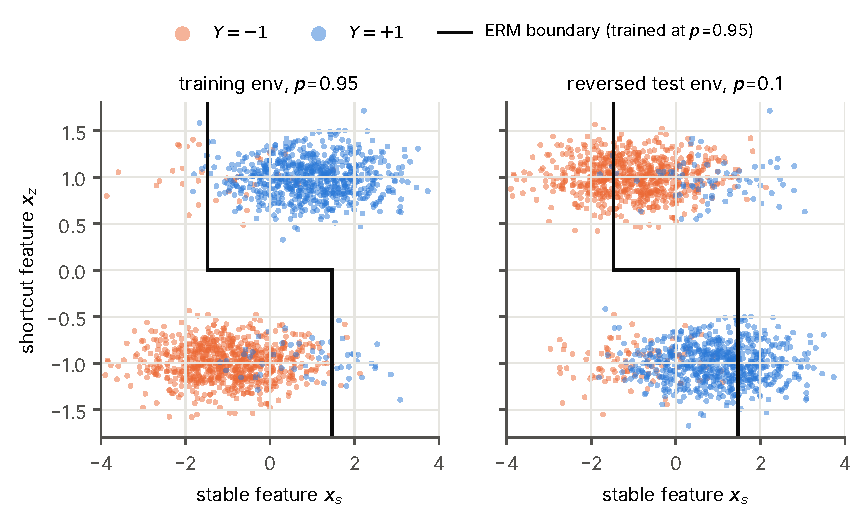
\includegraphics[width=0.78\linewidth]{fig0_data_scatter.pdf}
  \caption{Synthetic data. Left: training environment ($p=0.95$); the shortcut $x_z$ separates the
  classes almost perfectly. Right: reversed environment. The black line is the decision boundary of
  the training environment's Bayes rule (\cref{prop:bayes}); it sends most reversed-environment
  points to the wrong side.}
  \label{fig:scatter}
\end{figure}

\paragraph{Methods.} All methods are $\ell_2$-regularized logistic regression on standardized
features \cite{pedregosa2011sklearn}, with $C\in\{0.01,0.1,1,10,100\}$ chosen by validation log loss
and threshold $0.5$. \textbf{ERM} uses unit weights. \textbf{Group balanced (GB)} uses weight
$n/(4n_g)$ for an example in group $g=(Y,A)$, so each of the four groups carries total weight $n/4$.
\textbf{Stable only} uses $X_s$ alone and serves as a reference that knows which feature is stable.
For E3 we interpolate,
\begin{equation}
  w_i(\alpha) = (1-\alpha) + \alpha\,\frac{n}{4\,n_{g(i)}},
  \label{eq:walpha}
\end{equation}
so $\alpha=0$ is ERM and $\alpha=1$ is GB. Metrics are accuracy in each test environment and
worst-group accuracy over the four groups.

\section{Theory}
\label{sec:theory}

Proofs are in \cref{app:proofs}. Write $\Phi$ for the standard normal CDF and
$c_p=\log\frac{p}{1-p}$.

\begin{proposition}[Bayes rule and its accuracy]
\label{prop:bayes}
In environment $p$ the Bayes log-odds is $2x_s + g_p(x_z)$, where
$g_p(z)=\log\frac{p\,\phi_\sigma(z-1)+(1-p)\phi_\sigma(z+1)}{p\,\phi_\sigma(z+1)+(1-p)\phi_\sigma(z-1)}$
and $\phi_\sigma$ is the $N(0,\sigma^2)$ density. The rule $h_p(x)=\sign\big(2x_s+c_p\,\sign(x_z)\big)$
has accuracy in an environment with correlation $q$
\begin{equation}
  \Acc(p,q) = q\,\Phi\!\left(1+\tfrac{c_p}{2}\right) + (1-q)\,\Phi\!\left(1-\tfrac{c_p}{2}\right)
  \label{eq:acc}
\end{equation}
up to an additive error at most $\Phi(-1/\sigma)=\Phi(-5)<3\times10^{-7}$. Numerically, $h_p$ and the
exact Bayes rule differ in accuracy by less than $10^{-4}$ in all our settings.
\end{proposition}

Two consequences follow. (i) The optimal predictor of the training environment uses the shortcut,
with weight $c_p$ (2.94 at $p=0.95$) compared with weight 2 on $x_s$; this is optimal, not a failure
of optimization. (ii) $\Acc(p,q)$ is linear in $q$ and does not depend on $n$. Any consistent
learner converges to $h_p$, or for logistic regression to the population logistic minimizer
$\beta(p)$, whose OOD accuracy is likewise fixed by $p$ and $q$ (\cref{app:linear}). More data
therefore reduces variance around a predictor that is itself wrong for $q<p$. Using a stable-only
predictor gives $\Phi(1)=0.841$ in every environment; by \eqref{eq:acc}, ERM beats it only when
$q > 0.55$, $0.66$ and $0.78$ for $p=0.6$, $0.8$ and $0.95$ respectively.

\begin{proposition}[Reweighting changes the environment]
\label{prop:reweight}
Let $\hat p$ be the fraction of training examples with $A=Y$, and assume the two labels are balanced
within each value of $A=Y$ and $A\neq Y$. Then the $w(\alpha)$-weighted empirical distribution has the
same within-group distributions as the training data and group masses of an environment with
correlation
\begin{equation}
  p_\alpha = \hat p - \alpha\left(\hat p-\tfrac12\right).
  \label{eq:palpha}
\end{equation}
The weights are non-negative if and only if $0\le\alpha\le 2\hat p/(2\hat p-1)$, in which range
$p_\alpha$ covers $[0,\hat p]$. In the population, weighted ERM therefore has the same minimizer as
unweighted ERM in environment $p_\alpha$.
\end{proposition}

The key step is that total weight is preserved: $\hat p\,w_{\text{maj}}+(1-\hat p)\,w_{\text{min}}=1$
for every $\alpha$, so the weighted majority mass is exactly $\hat p\,w_{\text{maj}}=p_\alpha$.

\begin{corollary}[Optimal reweighting for a known test environment]
\label{cor:alpha}
For a test environment with correlation $q\in[0,p]$, the choice
$\alpha^*=\frac{p-q}{p-1/2}$ makes the weighted training distribution equal to the test distribution,
so the weighted population risk equals the test risk. In the Gaussian model the resulting
classifier is the Bayes rule of the test environment and attains $\Acc(q,q)$; for $q=0.1$ this is
$0.928$, compared with $0.841$ for GB ($\alpha=1$). The whole frontier is
$\alpha\mapsto\big(\Acc(p_\alpha,p),\,\Acc(p_\alpha,q)\big)$.
\end{corollary}

\Cref{cor:alpha} is importance weighting \cite{shimodaira2000} written in group form; what the
model adds is that every point on the frontier has a closed form, and that \emph{over-balancing}
($\alpha>1$) is the correct choice when the shortcut is expected to reverse.

\section{Experiments}
\label{sec:experiments}

\subsection{E1/E2: more data does not help, balancing does}

\Cref{tab:e1} reports $n=8000$; the predictions use the population logistic minimizer
(\cref{app:linear}). ERM matches the theory in every cell, GB and stable-only both sit at $\Phi(1)$,
and worst-group accuracy of ERM falls to $0.29$ at $p=0.95$. Paired over seeds at $p=0.95$, GB
minus ERM is $-0.115$ ID (95\% bootstrap CI $[-0.119,-0.111]$) and $+0.454$ in the reversed
environment ($[0.445, 0.464]$).

\begin{table}[t]
  \caption{Test accuracy at $n=8000$ (mean $\pm$ s.d.\ over 10 seeds) and the large-sample prediction
  in brackets. WGA: worst-group accuracy on the ID test set.}
  \label{tab:e1}
  \centering
  \small
  \begin{tabular}{llcccc}
    \toprule
    $p$ & Method & ID & No correlation & Reversed & WGA \\
    \midrule
    0.60 & ERM & $.846\pm.004$ [.846] & $.836\pm.002$ [.837] & $.797\pm.005$ [.799] & .781 \\
         & GB  & $.842\pm.004$ [.841] & $.842\pm.003$ [.841] & $.840\pm.005$ [.841] & .832 \\
    0.80 & ERM & $.885\pm.003$ [.886] & $.787\pm.004$ [.790] & $.659\pm.006$ [.660] & .615 \\
         & GB  & $.840\pm.004$ [.841] & $.842\pm.003$ [.841] & $.840\pm.004$ [.841] & .830 \\
    0.95 & ERM & $.958\pm.002$ [.958] & $.654\pm.011$ [.660] & $.386\pm.014$ [.394] & .293 \\
         & GB  & $.842\pm.007$ [.841] & $.842\pm.003$ [.841] & $.840\pm.008$ [.841] & .823 \\
    \midrule
    all  & Stable only & $.841\pm.004$ & $.842\pm.003$ & $.841\pm.004$ & .824 \\
    \bottomrule
  \end{tabular}
\end{table}

\Cref{fig:n} shows the role of $n$. For ERM at $p=0.95$, reversed-environment accuracy is
$0.371$, $0.392$ and $0.386$ at $n=500$, $2000$ and $8000$: the standard deviation over seeds shrinks
from $0.051$ to $0.014$, but the mean stays at the predicted $0.394$. The learned shortcut weight
(\cref{app:extra}, \cref{fig:coef}) is already close to its population value at $n=500$.
\Cref{fig:surface} (right) compares all 81 (method, $p$, $n$, environment) cells with the prediction:
the mean absolute gap is $0.0018$ and the largest is $0.023$, at $n=500$.

\begin{figure}[t]
  \centering
  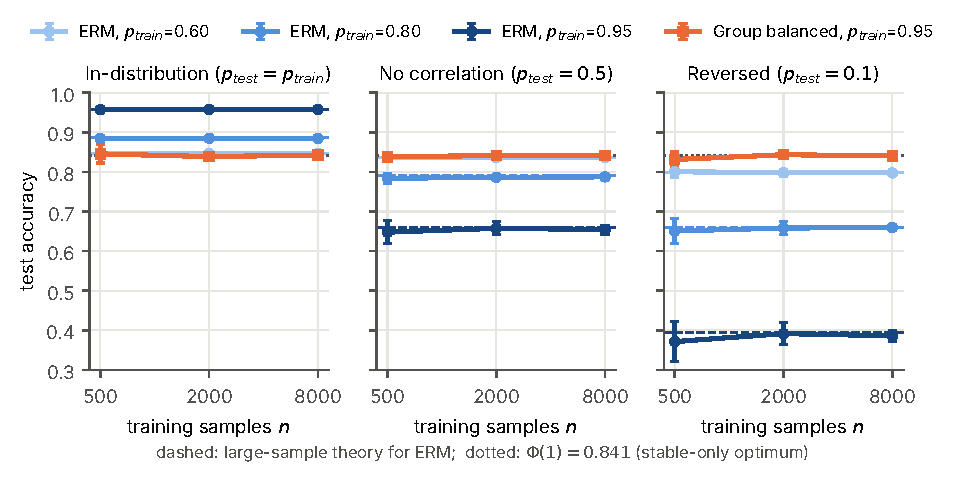
\includegraphics[width=\linewidth]{fig1_n_effect.pdf}
  \caption{Accuracy against training size. Dashed lines: large-sample prediction for ERM. Error bars:
  s.d.\ over 10 seeds. ERM accuracy does not change with $n$ in any environment.}
  \label{fig:n}
\end{figure}

\begin{figure}[t]
  \centering
  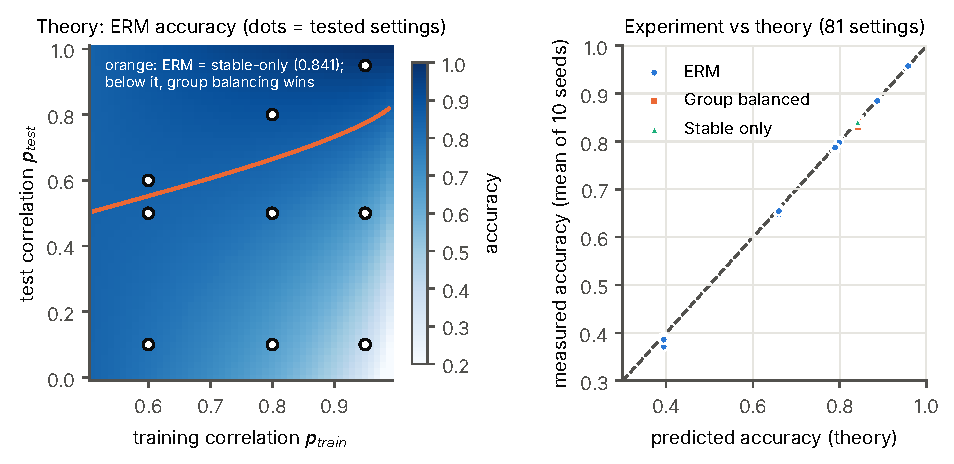
\includegraphics[width=\linewidth]{fig2_theory_surface.pdf}
  \caption{Left: predicted ERM accuracy over training and test correlation; below the orange curve,
  balancing beats ERM. Right: measured versus predicted accuracy for all 81 settings.}
  \label{fig:surface}
\end{figure}

\subsection{E3: the reweighting frontier}

We train with $\alpha\in\{0,0.25,0.5,0.75,1,1.25,1.5\}$ and $\alpha^*$ for $q=0.1$, for each
$p$, $n\in\{500,8000\}$ and 10 seeds. \Cref{fig:frontier} overlays the measured accuracies on the
frontier of \cref{cor:alpha}. The points follow the curve, including $\alpha>1$: at $p=0.95$,
$\alpha^*=1.89$ reaches $0.926$ in the reversed environment against a prediction of $0.928$.

\paragraph{Validation must be reweighted too.} If $C$ is chosen by unweighted log loss on the ID
validation set, the selection step undoes part of the reweighting: for $\alpha>1$ it picks the
strongest regularization ($C=0.01$ in all 10 seeds at $\alpha^*$ for $p=0.95$, $n=8000$), and the mean absolute gap to the
prediction rises from $0.0018$ to $0.0048$ (maximum $0.059$) at $n=8000$, and to $0.010$
(maximum $0.14$) at $n=500$. Using the same weights $w(\alpha)$ in the validation loss, which estimates
the risk under $p_\alpha$, restores agreement (maximum gap $0.013$ at $n=8000$). All E3 results above
use the weighted rule; the unweighted runs (another 480 models) are kept in \texttt{results/e3\_alpha.csv}.

\begin{figure}[t]
  \centering
  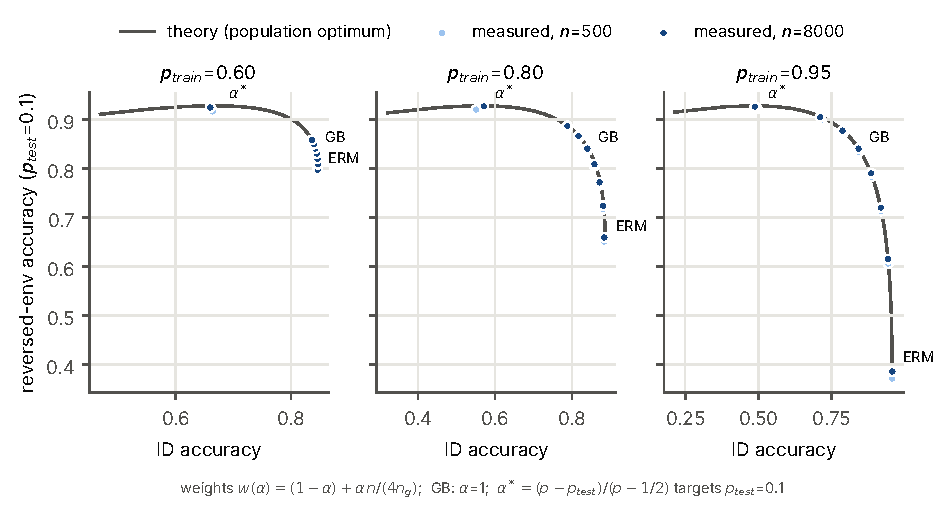
\includegraphics[width=\linewidth]{fig5_frontier.pdf}
  \caption{ID accuracy against reversed-environment accuracy as $\alpha$ varies. Curve: population
  prediction (\cref{cor:alpha}); points: means over 10 seeds. ERM: $\alpha=0$; GB: $\alpha=1$;
  $\alpha^*$ targets $p_{\text{test}}=0.1$.}
  \label{fig:frontier}
\end{figure}

\subsection{E4: an image-level check on MNIST}

\paragraph{Construction.} We keep MNIST digits 0 and 1 \cite{lecun1998mnist} (12\,665 training images,
10\% held out for validation; 2115 test images). As in Colored MNIST \cite{arjovsky2019irm}, the
observed label is the digit flipped with probability $0.25$, so the digit predicts $Y$ with accuracy
$Q=0.75$ in every environment. The shortcut is a $4\times4$ patch in the top-left corner, light
($0.25$) for $A=-1$ and dark ($0.75$) for $A=+1$, with $P(A=Y)=0.95$ in training
(\cref{fig:mnist}a). A two-layer CNN is trained with Adam (learning rate $10^{-3}$, batch 128,
10 epochs, best epoch by $w(\alpha)$-weighted validation loss) for 3 seeds.

\paragraph{Prediction.} Since the CNN recognizes 0 versus 1 almost perfectly, the task reduces to two
binary cues that agree with $Y$ independently, the digit with probability $Q$ and the marker with
probability $p$. The Bayes rule follows whichever cue has the larger log-odds weight, $c_Q$ or
$|c_p|$. By \cref{prop:reweight}, reweighting moves the training environment to $p_\alpha$, so the
model should follow the marker while $p_\alpha>0.75$ ($\alpha<0.44$), the digit while
$0.25<p_\alpha<0.75$, and the inverted marker when $p_\alpha<0.25$ ($\alpha>1.56$). The predicted
accuracies are $p_{\text{test}}$, $0.75$ and $1-p_{\text{test}}$ respectively (\cref{app:proofs}).

\paragraph{Result.} \Cref{fig:mnist}b shows the three regimes. ERM agrees with the marker on 100\% of
test images and scores $0.950/0.492/0.100$ in the three environments (predicted $0.95/0.50/0.10$);
its worst-group accuracy is 0. GB gives $0.757/0.752/0.741$ (predicted $0.75$), and $\alpha^*$ gives
$0.883$ in the reversed environment (predicted $0.90$). Near the two switching points
($\alpha=0.4, 0.5, 1.5$) the change is gradual rather than a jump, with large seed-to-seed variance:
the CNN is not exactly the two-cue Bayes rule, and with finite data the two cues have similar
weights there.

\begin{figure}[t]
  \centering
  \begin{subfigure}[b]{0.43\linewidth}
    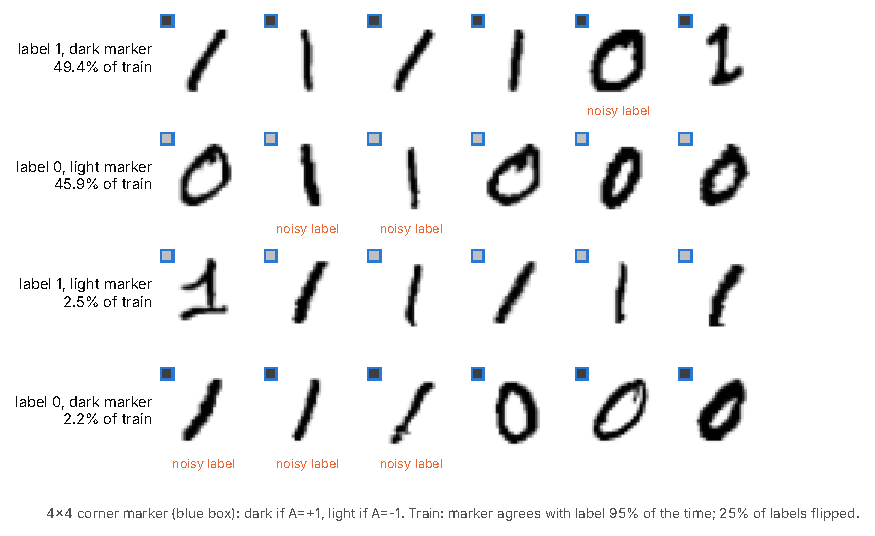
\includegraphics[width=\linewidth]{fig0_mnist_examples.pdf}
    \caption{Training images by (label, marker) group.}
  \end{subfigure}\hfill
  \begin{subfigure}[b]{0.55\linewidth}
    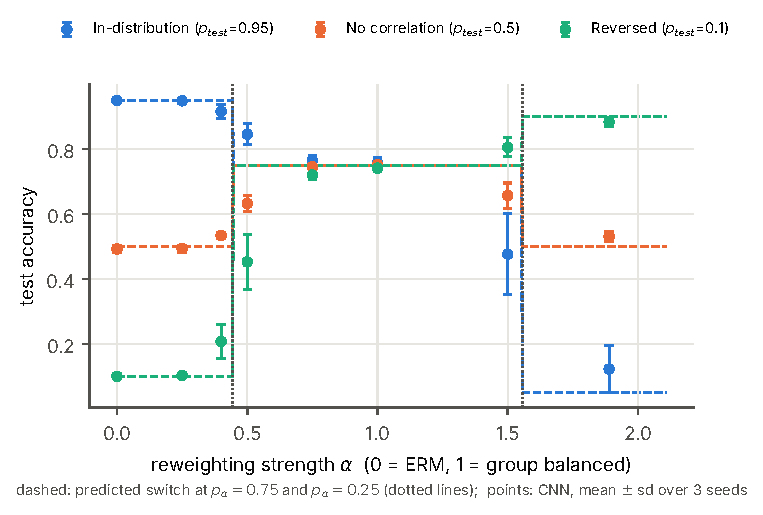
\includegraphics[width=\linewidth]{fig6_mnist.pdf}
    \caption{Accuracy against $\alpha$; dashed: prediction.}
  \end{subfigure}
  \caption{MNIST with a corner marker. (a) The marker (blue box) agrees with the label in 95\% of
  training images; 25\% of labels are flipped. (b) Mean $\pm$ s.d.\ over 3 seeds.}
  \label{fig:mnist}
\end{figure}

\section{Discussion and limitations}
\label{sec:discussion}

\paragraph{What we learned.} When a shortcut is reliable in the training data, relying on it is the
optimal thing to do for that data; the failure is a mismatch between environments, so more data from
the same environment cannot fix it. Group reweighting works because it is a change of environment,
and in our model the size of that change is linear in the reweighting strength. This gives a precise
cost of robustness (for $p=0.95$, $0.117$ ID accuracy for GB) and shows that the usual choice $\alpha=1$
is optimal only for $p_{\text{test}}=0.5$.

\paragraph{Limitations.} The theory assumes known group labels, a binary attribute, conditionally
independent features and a known test correlation for $\alpha^*$; real spurious attributes are rarely
all of these. The Gaussian model is chosen so the predictions are exact, which limits external
validity. E4 tests one image construction, one architecture and 3 seeds, and its prediction is
qualitative near the switching points. We did not compare with Group DRO \cite{sagawa2020dro} or
with methods that infer groups. Uncertainty intervals reflect seed variation in this simulation only.

\section{Conclusion}
In a model where the answer can be computed, the two common remedies for shortcut learning behave
very differently: more data does not change OOD accuracy at all, while group reweighting moves the
model along a closed-form frontier whose optimal point depends on the test environment. The same
identity predicts where a CNN on MNIST switches cues.

\paragraph{Code.} \url{https://github.com/Er1cShi/JHU_ML_Course_Final_Project}; every number and
figure is produced by the scripts listed in \cref{app:extra}.

\paragraph{Author contributions.} [Author 1] designed and ran all code and experiments and prepared the
slides. [Author 2] and [Author 3]: [to be filled in, e.g.\ presentation, literature
review, proof checking, writing]. \textit{[Edit before submission.]}

\paragraph{AI-use statement.} We used Claude (Anthropic), through the Claude Code agent in a project
workspace, throughout the project. It decomposed the project from the course's topic description,
wrote the data generator, training and analysis code, derived the propositions in
\cref{sec:theory}, ran the experiments, produced the figures and drafted this report. Its
derivations were checked by independent numerical routes in the code: Monte Carlo against
\eqref{eq:acc}, numerical integration against the sign approximation, and a 2-million-sample fit for
the population logistic minimizer. Human judgment chose the topic, asked for the MNIST experiment
and the closed-form frontier as the originality direction, and decided what to report.
\textit{[Edit before submission: describe which derivations and citations you checked by hand,
what you changed or rejected, and how you prompted.]}

{\small
\bibliographystyle{plainnat}
\bibliography{references}
}

\newpage
\appendix

\section{Proofs}
\label{app:proofs}

\paragraph{Proof of \cref{prop:bayes}.} Given $Y=y$, $X_s\sim N(y,1)$ and $X_z$ is the mixture
$p\,N(y,\sigma^2)+(1-p)\,N(-y,\sigma^2)$, independent of $X_s$. With $P(Y=1)=\tfrac12$,
\[
\log\frac{P(Y=1\mid x)}{P(Y=-1\mid x)}
=\log\frac{\phi(x_s-1)}{\phi(x_s+1)}+\log\frac{p\,\phi_\sigma(x_z-1)+(1-p)\phi_\sigma(x_z+1)}{p\,\phi_\sigma(x_z+1)+(1-p)\phi_\sigma(x_z-1)}
=2x_s+g_p(x_z).
\]
When $x_z$ is far from 0 relative to $\sigma$, one mixture component dominates and
$g_p(x_z)\approx c_p\,\sign(x_z)$, which gives $h_p$. For its accuracy in environment $q$, condition on
$Y=1$ (the case $Y=-1$ is symmetric). Then $\sign(X_z)=A$ unless $|\sigma\varepsilon_z|>1$, which has
probability at most $2\Phi(-1/\sigma)$ and changes the accuracy by at most $\Phi(-1/\sigma)$ on
average over the two values of $A$. If $A=1$ (probability $q$), $h_p$ is correct iff
$2X_s+c_p>0$, i.e.\ $X_s>-c_p/2$, which has probability $\Phi(1+c_p/2)$ since $X_s\sim N(1,1)$. If
$A=-1$ (probability $1-q$), it is correct iff $X_s>c_p/2$, with probability $\Phi(1-c_p/2)$. Summing
gives \eqref{eq:acc}. The exact Bayes rule replaces $c_p\,\sign(x_z)$ by $g_p(x_z)$; integrating over
$x_z$ numerically (\texttt{theory.acc\_bayes\_exact}) agrees with \eqref{eq:acc} to four decimals in all
our settings. \hfill$\square$

\paragraph{Proof of \cref{prop:reweight}.} Let $n_g$ be the group counts. Under the balance assumption,
each of the two majority groups $(y,A=y)$ has $n_g=\hat p\,n/2$ and each minority group has
$n_g=(1-\hat p)\,n/2$, so $n/(4n_g)$ equals $1/(2\hat p)$ and $1/(2(1-\hat p))$ respectively, and
\[
w_{\text{maj}}=(1-\alpha)+\frac{\alpha}{2\hat p},\qquad
w_{\text{min}}=(1-\alpha)+\frac{\alpha}{2(1-\hat p)}.
\]
The weighted empirical distribution puts mass $\hat p\,w_{\text{maj}}$ on the majority groups and
$(1-\hat p)\,w_{\text{min}}$ on the minority groups, and does not change the distribution within a
group. Since $\hat p\,w_{\text{maj}}+(1-\hat p)\,w_{\text{min}}=(1-\alpha)+\alpha/2+\alpha/2=1$, these are
proper probabilities, and the majority mass is $\hat p(1-\alpha)+\alpha/2=\hat p-\alpha(\hat p-\tfrac12)$.
Labels remain balanced by symmetry, and within-group distributions do not depend on $p$ in
\eqref{eq:gen}, so the weighted distribution is that of environment $p_\alpha$. Non-negativity:
$w_{\text{min}}\ge0$ for all $\alpha\ge0$, and $w_{\text{maj}}\ge0$ iff
$\alpha\le 2\hat p/(2\hat p-1)$, at which point $p_\alpha=0$. In the population ($\hat p=p$) the
weighted risk $\E[w(\alpha)\,\ell]$ equals the unweighted risk in environment $p_\alpha$, so the two
minimizers coincide. Without exact balance the same argument applies group by group with
$p_\alpha$ defined from the weighted group masses. \hfill$\square$

\paragraph{Proof of \cref{cor:alpha}.} Solving $p_\alpha=q$ in \eqref{eq:palpha} gives
$\alpha^*=(p-q)/(p-\tfrac12)$, which lies in the non-negative range for $q\in[0,p]$. The weighted
training distribution is then the test distribution, so the weighted population risk of any predictor
equals its test risk, and its minimizer over a class containing the Bayes rule is the Bayes rule of
environment $q$, with accuracy $\Acc(q,q)$ by \cref{prop:bayes}. \hfill$\square$

\paragraph{Two-cue model for E4.} Let $\tilde d,\tilde a\in\{\pm1\}$ indicate whether the digit and
the marker agree with $Y$; they are independent given $Y$, with $P(\tilde d=1)=Q$ and
$P(\tilde a=1)=r$ in environment $r$. The Bayes rule predicts the label favoured by
$c_Q\,\tilde d+c_r\,\tilde a$, i.e.\ it follows the marker if $|c_r|>c_Q$ (inverted if $r<\tfrac12$)
and the digit otherwise. Following the marker gives accuracy $q$ in a test environment $q$, following
the digit gives $Q$, and following the inverted marker gives $1-q$. With $r=p_\alpha$, the switches are
at $p_\alpha=Q$ and $p_\alpha=1-Q$, i.e.\ $\alpha=(p-Q)/(p-\tfrac12)=0.44$ and
$\alpha=(p-1+Q)/(p-\tfrac12)=1.56$ for $p=0.95$, $Q=0.75$. \hfill$\square$

\section{Population optimum of the linear model}
\label{app:linear}

Logistic regression is linear in $x$ while the Bayes log-odds is a step function of $x_z$, so the
population logistic minimizer $\beta(p)=(b_0,b_s,b_z)$ differs slightly from $(0,2,c_p)$. We compute it
by an essentially unregularized fit on $2\times10^6$ samples: $b_z=0.39,1.34,2.90$ for
$p=0.6,0.8,0.95$, against $c_p=0.41,1.39,2.94$, with $b_s\approx2.0$. For any linear rule, the score
given $(Y,A)=(y,a)$ is Gaussian with mean $b_0+y\,b_s+a\,b_z$ and variance $b_s^2+\sigma^2b_z^2$, so its
accuracy in environment $q$ is an exact average of four normal CDF values
(\texttt{theory.acc\_linear}). These are the predictions in \cref{tab:e1} and the dashed lines in
\cref{fig:n}. The OOD accuracy of $\beta(p)$ depends only on $p$ and $q$, and by standard consistency
of M-estimators the fitted coefficients converge to $\beta(p)$ as $n\to\infty$.

\section{Additional results and implementation}
\label{app:extra}

\begin{figure}[h]
  \centering
  \begin{subfigure}[b]{0.48\linewidth}
    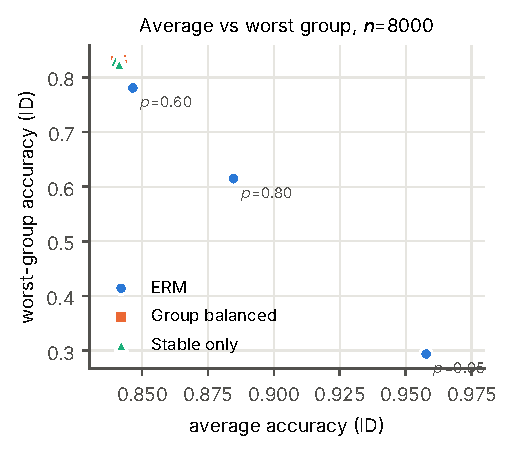
\includegraphics[width=\linewidth]{fig3_tradeoff.pdf}
    \caption{Average versus worst-group accuracy.}
  \end{subfigure}\hfill
  \begin{subfigure}[b]{0.48\linewidth}
    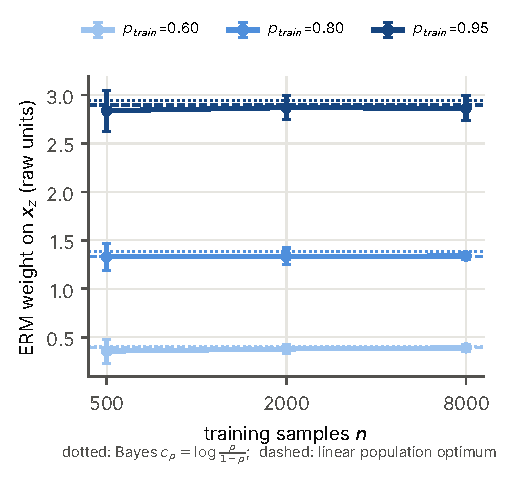
\includegraphics[width=\linewidth]{fig4_coef.pdf}
    \caption{Learned shortcut weight.}
    \label{fig:coef}
  \end{subfigure}
  \caption{(a) ID test set, $n=8000$. (b) ERM weight on $x_z$ in raw units, mean $\pm$ s.d.\ over 10
  seeds; it is close to the population value at every $n$.}
\end{figure}

\begin{figure}[h]
  \centering
  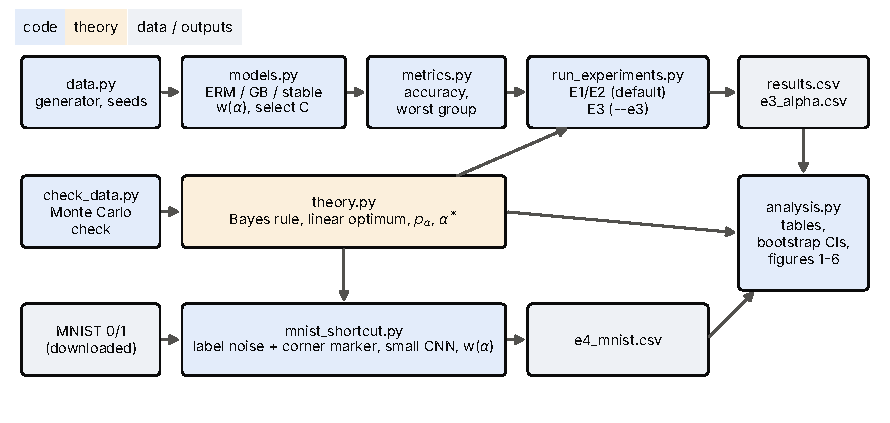
\includegraphics[width=0.9\linewidth]{fig0_pipeline.pdf}
  \caption{Code structure. Each experiment writes a CSV; \texttt{analysis.py} produces all tables and
  figures.}
\end{figure}

\paragraph{Implementation.} Logistic regression uses scikit-learn's L-BFGS solver (tolerance
$10^{-6}$, at most 1000 iterations); all 1350 candidate fits in E1 and all E3 fits converged.
Standardization is fitted on training data only. Seeds 0--9 index the training pool, validation and
test sets; smaller training sets are prefixes of the pool. Bootstrap intervals resample the 10 seed-level
paired differences 2000 times. E1 takes about 20\,s and E3 about 1\,min on a laptop CPU; E4 takes
about 4\,min.

\end{document}
